\subsubsection{Teori}
\underline{\textbf{Send-and-Wait protokol}}
\newline
Stop-and-Wait er et special tilfælde af Go-Back-N.
Stop-and-Wait har to sekvensnumre, mens Go-Back-N har flere
\newline
I stop-and-wait protokollen tilføjes en fejl mekaisme, hvor der tilføjes redundante bit for at finde og rette fejl i sendte pakker, dette gøres ved hjælp af CRC checket, som forklares senere.
\newline
Ved hjælp af sekvensnummerering af pakkerne, er modtageren i stand til at konstatere om den modtagne pakke er den korrekte, eller om den har et forkert nummer i forhold til rækkefølgen.
\newline
Automatic repeat request (ARQ) benyttes når mistede eller fejlbehæftede pakker skal retransmitteres. Pakker retransmitteres hvis en ny ACK ikke er modtaget inden timeren udløber.
\newline
\textbf{Open}
\newline
Som der ses i figur \ref{fig:open}, sendes Segment 0, når Sender er aktiv. Hvis Modtager er aktiv oprettes der forbindelse og Modtager sender ACK 0 (acknowledgement 0) og Sender ved at der er forbindelse.
\newline
Hvis Modtager derimod ikke er aktiv vil Sender ikke modtage ACK 0, og Sender vil derfor vente 10 sekunder før igen at sende Segment 0. Dette vil Sender gøre op til tre gange, hvis nødvendigt.
\begin{figure}[ht]
	\centering
	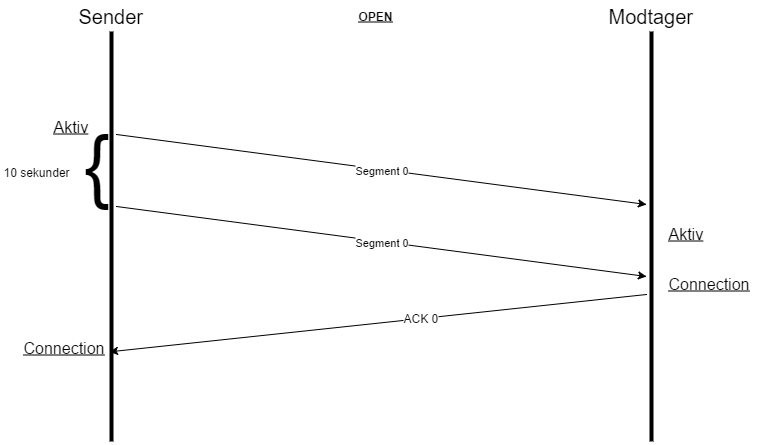
\includegraphics[width=15cm,height=25cm,keepaspectratio]{pictures/Open.png}
	\caption{Open}
	\label{fig:open}
\end{figure}

\hfill \break
\textbf{Stream}
\newline
Stream delen, som kan ses på figur \ref{fig:stream}, er den del hvor data sendes.
\newline
Her sender Sender først Segment 1. Hvis dette er blevet korrekt modtaget vil Modtager sende ACK 1.
Dette vil forstætte indtil Close. 

\begin{figure}[ht]
	\centering
	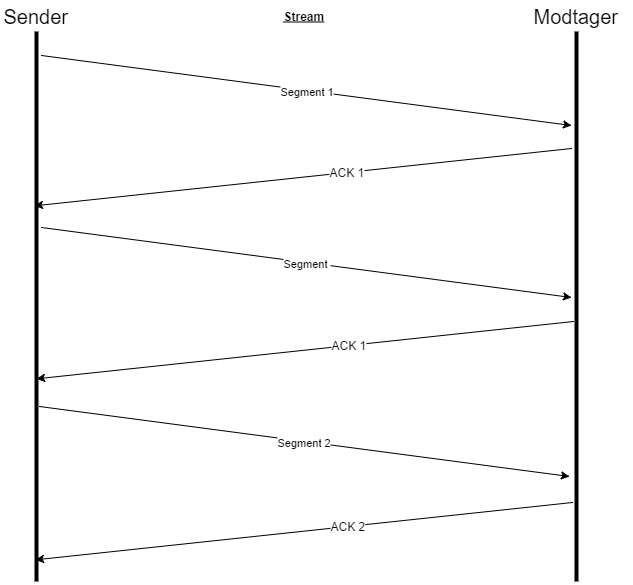
\includegraphics[width=15cm,height=25cm,keepaspectratio]{pictures/Stream.png}
	\caption{Stream}
	\label{fig:stream}
\end{figure}

\hfill \break
\hfill \break
\textbf{Close}
\newline
Close delen kan ses på figur \ref{fig:close}.
\newline
I denne del gør Sender Modtager opmærksom på at der ikke sendes mere.

\begin{figure}[ht]
	\centering
	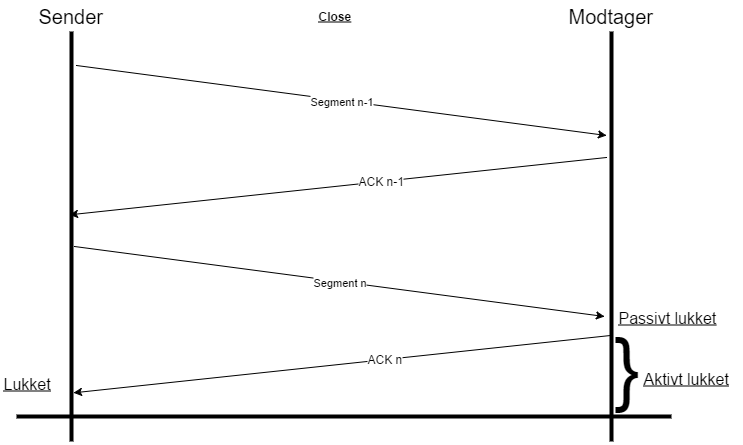
\includegraphics[width=15cm,height=25cm,keepaspectratio]{pictures/Close.png}
	\caption{Close}
	\label{fig:close}
\end{figure}

\hfill \break
\hfill \break
\hfill \break
\hfill \break
\underline{\textbf{Flag}}
\newline
I projekt koden er der benyttet tre flag til at fortælle om beskeden er en probe, accept, eller sidste besked.
Der benyttes 3 bit, til at definere flaget. 001 er probe, 010 er accept og 100 er last.
\hfill \break
\newline
Der blev valgt ikke at bruge fuld dublex, da dette kræver tråde og flere bytes.